\documentclass{ifacconf}

\usepackage{natbib}            % you should have natbib.sty
\usepackage[utf8]{inputenc}    % Eingabe von Umlauten im Editor, dieser sollte dann auch auf utf8 Encoding eingestellt sein
\usepackage{graphicx}          % Include this line if your 
                               % document contains figures,
%\usepackage[dvips]{epsfig}    % or this line, depending on which
                               % you prefer.
                               
\usepackage{units}

% for German
% \usepackage{ngerman}           % neue Deutsche Rechtschreibung, Silbentrennung
% \usepackage[T1]{fontenc}       % Trennung mit Umlauten

% to include tikz pictures of figure created with matlab2tikz, see also file ``plotFigureTest.m''
\usepackage{tikz}
\usepackage{pgfplots}
\pgfplotsset{compat=newest}  % use newest version of pgfplots
\usepackage{amsmath}  % useful for math

% to include the legend into the caption. The commands are
%\mlLineLegend{red}
%\mlLineLegendDashed{red}
%\mlLineLegendDotted{red}
%\mlLineLegendDashDotted{red}
%\mlPointLegend{red}
\newlength{\mlLegendThickness}
\setlength{\mlLegendThickness}{0.4mm}
\newlength{\mlLegendHeight}
\setlength{\mlLegendHeight}{0.6ex}
\newcommand{\mlLineLegend}[1]{\mbox{\color{#1}
\protect\rule[\mlLegendHeight]{3mm}{\mlLegendThickness}\hspace*{-1mm}
}}
\newcommand{\mlLineLegendDashed}[1]{\mbox{\color{#1}
\protect\rule[\mlLegendHeight]{1.5mm}{\mlLegendThickness}\hspace*{0mm}
\protect\rule[\mlLegendHeight]{1.5mm}{\mlLegendThickness}\hspace*{-1mm}
}}
\newcommand{\mlLineLegendDotted}[1]{\mbox{\color{#1}
\protect\rule[\mlLegendHeight]{0.4mm}{\mlLegendThickness}\hspace*{0mm}
\protect\rule[\mlLegendHeight]{0.4mm}{\mlLegendThickness}\hspace*{0mm}
\protect\rule[\mlLegendHeight]{0.4mm}{\mlLegendThickness}\hspace*{0mm}
\protect\rule[\mlLegendHeight]{0.4mm}{\mlLegendThickness}\hspace*{-1mm}
}}
\newcommand{\mlLineLegendDashDotted}[1]{\mbox{\color{#1}
\protect\rule[\mlLegendHeight]{1.5mm}{\mlLegendThickness}\hspace*{0mm}
\protect\rule[\mlLegendHeight]{0.4mm}{\mlLegendThickness}\hspace*{0mm}
\protect\rule[\mlLegendHeight]{1.5mm}{\mlLegendThickness}\hspace*{0mm}
\protect\rule[\mlLegendHeight]{0.4mm}{\mlLegendThickness}\hspace*{-1mm}
}}
\newcommand{\mlPointLegend}[1]{\mbox{\color{#1}
\protect\rule[\mlLegendHeight]{0.4mm}{\mlLegendThickness}\hspace*{-0.75mm}
}}

\begin{document}

\begin{frontmatter}

\title{Laborprotocol BMo2-1}


% include all authors, underline corresponding author
\author{E. Boateng,} 
\author{J. Qin} 
% \author{}

\begin{abstract}                          % Abstract of not more than 250 words.
This protocol for L1 and H1 is concerned with the experimental setup. A qualified model of the dynamics were derived and missing parameters of the model were identified.
\end{abstract}

\end{frontmatter}

\section{Work tasks}
First, to be familiar with the experimental setup. A strategy should be develpoed to solve the main task of the lab course. In addition, a system need to be modeled with an adequate precision and linearized.


\section{Simulation model of the helicopter}

In order to be able to design controllers during L2, the helicopter system has to be modeled. Because the complete model of the helicopter is very complicated, simplification of the model while keeping the model complexity within an acceptable range is necessary.

Figure 1 shows the simplified model with the corresponding
parameters.

Apply the law of angular momentum to the axes a,b and c, the following equations are derived.


\begin{align}	
&\Theta_a\ddot{\alpha} = -\cos(\beta)L_2\sin(\gamma)(F_f+F_b)\\
&\Theta_b\ddot{\beta} = \cos(\gamma)L_2(F_f+F_b)-\cos(\beta)(mL_1-ML_2)g\\
&\Theta_c\ddot{\gamma} = \frac{L_3}{2}(F_f-F_b)
\end{align}

$\Theta_a$, $\Theta_b$ and $\Theta_c$ are the moment of inertia with respect to the axes a,b and c. Their values can be calculated by the following equations.

\begin{align}
\Theta_a &= mL_1^2 + ML_2^2\\
\Theta_b &= mL_1^2 + ML_2^2\\
\Theta_c &= \frac{1}{6}m(\frac{L3}{2})^2
\end{align}


\begin{figure} % use \begin{figure*} for two-column figure
\begin{center} 
% the variable for the width of the figure which you created with matlab2tikz has to be defined and set
\newlength{\figurewidth} % ... defined
\setlength{\figurewidth}{0.8\columnwidth} % ...set 
% for details see file ``plotFigureTest.m''
%% This file was created by matlab2tikz.
%
%The latest updates can be retrieved from
%  http://www.mathworks.com/matlabcentral/fileexchange/22022-matlab2tikz-matlab2tikz
%where you can also make suggestions and rate matlab2tikz.
%
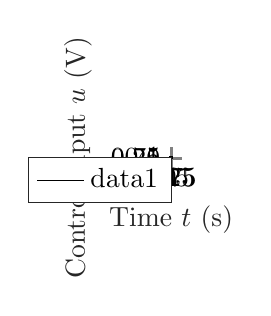
\begin{tikzpicture}

\begin{axis}[%
width=0.951\figurewidth,
height=0.75\figurewidth,
at={(0\figurewidth,0\figurewidth)},
scale only axis,
xmin=0,
xmax=1,
xtick={   0, 0.25,  0.5, 0.75,    1},
xlabel style={font=\color{white!15!black}},
xlabel={Time $t$ (s)},
ymin=0,
ymax=1,
ytick={   0, 0.25,  0.5, 0.75,    1},
ylabel style={font=\color{white!15!black}},
ylabel={Control input $u$ (V)},
axis background/.style={fill=white},
xmajorgrids,
ymajorgrids,
legend style={legend cell align=left, align=left, draw=white!15!black}
]
\addplot [color=black]
  table[row sep=crcr]{%
0	0\\
0.01	0.00999983333416666\\
0.02	0.0199986666933331\\
0.03	0.0299955002024957\\
0.04	0.0399893341866342\\
0.05	0.0499791692706783\\
0.06	0.0599640064794446\\
0.07	0.0699428473375328\\
0.08	0.0799146939691727\\
0.09	0.089878549198011\\
0.1	0.0998334166468282\\
0.11	0.109778300837175\\
0.12	0.119712207288919\\
0.13	0.129634142619695\\
0.14	0.139543114644236\\
0.15	0.149438132473599\\
0.16	0.159318206614246\\
0.17	0.169182349066996\\
0.18	0.179029573425824\\
0.19	0.188858894976501\\
0.2	0.198669330795061\\
0.21	0.2084598998461\\
0.22	0.218229623080869\\
0.23	0.227977523535188\\
0.24	0.237702626427135\\
0.25	0.247403959254523\\
0.26	0.257080551892155\\
0.27	0.266731436688831\\
0.28	0.276355648564114\\
0.29	0.285952225104836\\
0.3	0.29552020666134\\
0.31	0.305058636443443\\
0.32	0.314566560616118\\
0.33	0.324043028394868\\
0.34	0.333487092140814\\
0.35	0.342897807455451\\
0.36	0.35227423327509\\
0.37	0.361615431964962\\
0.38	0.370920469412983\\
0.39	0.380188415123161\\
0.4	0.389418342308651\\
0.41	0.398609327984423\\
0.42	0.40776045305957\\
0.43	0.416870802429211\\
0.44	0.425939465066\\
0.45	0.43496553411123\\
0.46	0.44394810696552\\
0.47	0.452886285379068\\
0.48	0.461779175541483\\
0.49	0.470625888171158\\
0.5	0.479425538604203\\
0.51	0.488177246882908\\
0.52	0.496880137843737\\
0.53	0.505533341204847\\
0.54	0.514135991653113\\
0.55	0.522687228930659\\
0.56	0.531186197920883\\
0.57	0.539632048733969\\
0.58	0.548023936791874\\
0.59	0.556361022912784\\
0.6	0.564642473395035\\
0.61	0.572867460100481\\
0.62	0.581035160537305\\
0.63	0.58914475794227\\
0.64	0.597195441362392\\
0.65	0.605186405736039\\
0.66	0.613116851973434\\
0.67	0.62098598703656\\
0.68	0.628793024018468\\
0.69	0.636537182221968\\
0.7	0.644217687237691\\
0.71	0.651833771021537\\
0.72	0.659384671971473\\
0.73	0.666869635003698\\
0.74	0.674287911628145\\
0.75	0.681638760023334\\
0.76	0.688921445110551\\
0.77	0.696135238627357\\
0.78	0.70327941920041\\
0.79	0.710353272417608\\
0.8	0.717356090899523\\
0.81	0.724287174370143\\
0.82	0.731145829726896\\
0.83	0.737931371109963\\
0.84	0.744643119970859\\
0.85	0.751280405140293\\
0.86	0.757842562895277\\
0.87	0.764328937025505\\
0.88	0.770738878898969\\
0.89	0.777071747526824\\
0.9	0.783326909627483\\
0.91	0.78950373968995\\
0.92	0.795601620036366\\
0.93	0.801619940883777\\
0.94	0.807558100405114\\
0.95	0.813415504789374\\
0.96	0.819191568300998\\
0.97	0.82488571333845\\
0.98	0.83049737049197\\
0.99	0.836025978600521\\
1	0.841470984807897\\
};
\addlegendentry{data1}

\end{axis}
\end{tikzpicture}% % inclusion of tikz-code
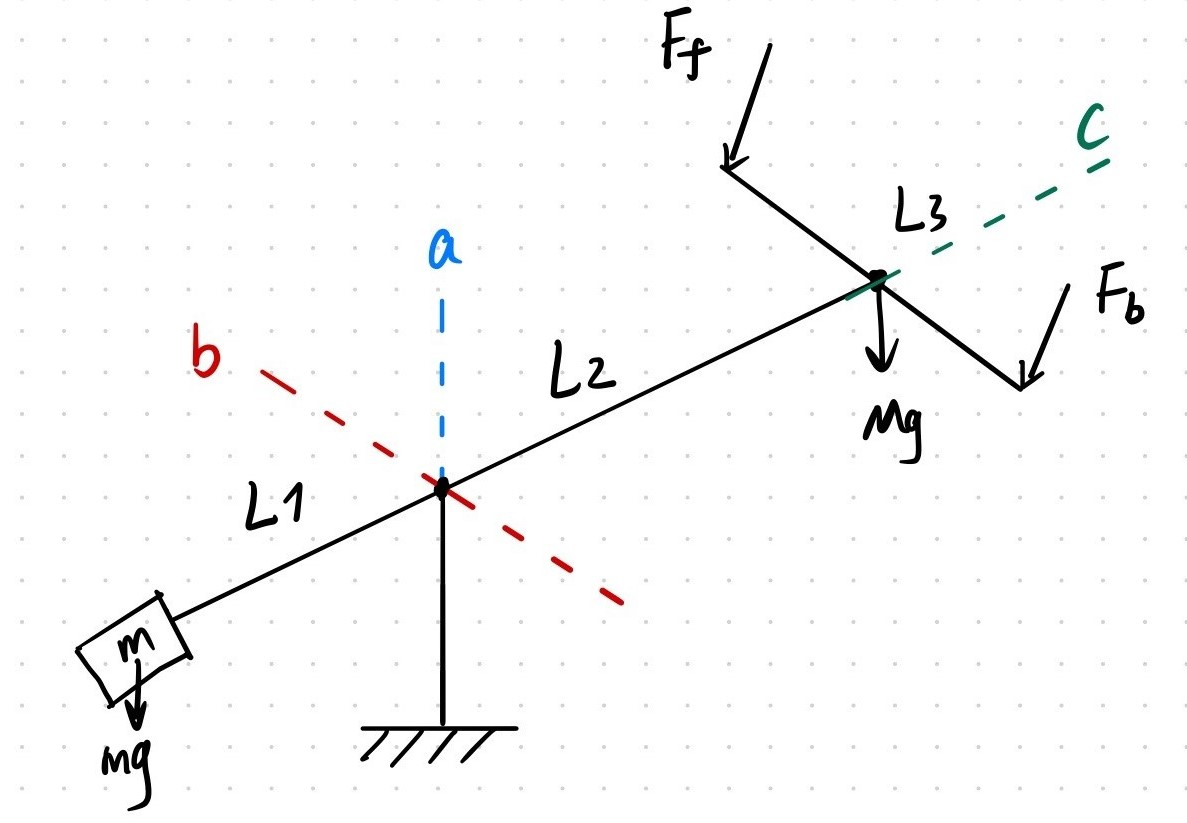
\includegraphics[width=\columnwidth]{model} % inclusion of pdf
\caption{simplified model of the helicopter}
\label{model}
		
\end{center}
\end{figure}


The state vector $x =\begin{bmatrix}
	\alpha&\beta&\gamma&\dot{\alpha}&\dot{\beta}&\dot{\gamma}
\end{bmatrix}^T$ and the input vector $u = \begin{bmatrix}
F_f&F_b
\end{bmatrix}^T$. Therefore, $\dot{x} = \begin{bmatrix}
\dot{\alpha}&\dot{\beta}&\dot{\gamma}&\ddot{\alpha}&\ddot{\beta}&\ddot{\gamma}
\end{bmatrix}^T$ can be displayed as follows.
\begin{equation}
\dot{x}=\begin{bmatrix}
	\dot{\alpha}\\
	\dot{\beta}\\
	\dot{\gamma}\\
	\frac{-\cos(\beta)L_2\sin(\gamma)(F_f+F_b)}{mL_1^2 + ML_2^2}\\
	\frac{\cos(\gamma)L_2(F_f+F_b)-\cos(\beta)(mL_1-ML_2)g}{mL_1^2 + ML_2^2}\\
	\frac{\frac{L_3}{2}(F_f-F_b)}{\frac{1}{6}m(\frac{L3}{2})^2}
\end{bmatrix}
\end{equation}

\section{LaTeX}

The protocols have to be typeset with \LaTeX. A good German introduction to \LaTeX can be found in \citep{hagenEinfuehrung}. An alternative in English is \citep{lshort}. A short guide concerning the mathematical part is given by \citep{mathGuide}.

\section{Submission}

Two files have to be submitted to the Praktikumskoordinator until 0:00 the day of the laboratory by uploading them into Ilias:
\begin{itemize}
\item A pdf-file of the protocol and
\item a zip-file containing all the relevant Matlab-files.
\end{itemize}
Every student has to be \emph{responsible} for the protocol and the zip-files \emph{once} during the course.

The protocol for every laboratory day has to contain
\begin{itemize}
\item a result protocol of the last laboratory, if applicable, 
\item a protocol of the preparation and 
\item a working plan for the next laboratory.
\end{itemize}
A template for the working plan can be found in Table~\ref{table:working plan}.
\begin{table*}
\caption{Working Plan for L2.}
\label{table:working plan}
\centering
\begin{tabular}{|c|c|p{4.5cm}|p{4.5cm}|p{4.5cm}|}
\hline
\bfseries Time & \bfseries Duration & \bfseries Goal & \bfseries Task & \bfseries Preparation\\ \hline \hline
14:00 & 30 min. & Test File to actuate motor & Create Quarc Simulink File & Read Quarc documentation \\ \hline
 &  &  &  &  \\ \hline
 &  &  &  &  \\ \hline
 &  &  &  &  \\ \hline
 &  &  &  &  \\ \hline
\end{tabular}
\end{table*}
Of the last laboratory day, a result protocol has to be written which is due one week after the laboratory.

To make your approach or results repeatable, comment all your Matlab-scripts and Simulink-files appropriately - preferably while working with them. Decide, which files and maybe also measurement data is necessary to repeat your results. Then, put all necessary files into one zip-file and upload it into Ilias. In the protocol you should reference the files where the information is only needed for repeatability. Furthermore, you should refer to the files while explaining your procedure. Thus, you don't have to include all information into the protocol.

You can write either in German or English. If you write in German, it is a good idea to include the packages ngerman, inputenc, and fontenc in the preamble of your tex-file.

\section{Structure}

In the title include your group description and the task the protocol is about. The group description follows the syntax \mbox{$IDDN$-$T$} with $I=\{A,B\}$ being the cycle number, $DD=\{Mo,We,Th\}$ the day, $N=\{1-4\}$ the group number and $T=\{1-5\}$ the task number. For example \mbox{IMo1-1}. Include all group members as authors. Underline the corresponding author. In the abstract, you should summarize the result within up to three sentences.

% if an error occurs here: go to the options of your editor and change the commands in the configuration panel corresponding to PDFLaTeX: add "-shell-escape" befor "%.tex"
%(e.g. Options --> Configure Texmaker --> Commands --> PDFLaTex --> "pdflatex -synctex=1 -interaction=nonstopmode -shell-escape %.tex" )

The structure on the section level has to be decided depending on the tasks. For the main sections, the structure can be similar to the problem-solving process:
\begin{itemize}
\item \emph{Work task} explaining the task and the goal.
\item \emph{Solution approach} describing the chosen solution to allow the reader to repeat and assess the solution.
\item \emph{Result} containing the observations and justified conclusions.
\item \emph{Critical comments} evaluating the approach including a comparison with the working plan. Furthermore the pros and cons should be discussed.
\end{itemize}

\section{Figures and Graphics}
All figures should be created as done in the Matlab-script ``plotFigureTest.m'' which can be found in Ilias. By following the procedure, the axis labels and ticks are in an appropriate size, the same \LaTeX-font is used, and the line thickness is adjusted resulting in a formally excellent figure. If you have plots in Simulink, export the data and create a Matlab figure. To label the axis, use words and not symbols. Write units in parentheses. E.g., write ``Control input $u$ (V)''. An easy and nice-looking way for the legend is to include it into the caption of the figure. See the tex-code for more details.


Graphics for the protocol can be made for example with the Open Source vector graphics editor Inkscape. Details can be found on \verb+http://inkscape.org/+.

\section{Final protocol}
\label{sec:finalProtocol}
At the end of the course a protocol over the whole laboratory has to be written. This final protocol may have up to 8 pages. The final protocol may be based on your other protocols and you can reuse parts of the other protocols. But the final protocol has to be self-contained and needs to have a comprehensible line of thought. 

The purpose of the final protocol is that the reader gets an idea of your whole solution. Therefore, it should contain the results of your work. To understand the results, you should also include your approaches on a more abstract level. For you, the final protocol is a chance to reflect the laboratory as a whole.


%\bibliographystyle{alpha}        % Include this if you use bibtex 
%\bibliography{autosam}           % and a bib file to produce the 
%\bibliography{autosam}
                                 % bibliography (preferred). The
                                 % correct style is generated by
                                 % Elsevier at the time of printing.

\begin{thebibliography}{3}

\bibitem[Jürgens and Feuerstack(2011)]{hagenEinfuehrung}
Jürgens,~M. and Feuerstack,~T. (2011).
\newblock \LaTeX - eine Einführung und ein bißchen mehr\dots .
\newblock Fernuniversität in Hagen, A/026/0911.
\newblock Available online from
\verb+http://www.fernuni-hagen.de/imperia/md+
\verb+/content/zmi_2010/a026_latex_einf.pdf+.

\bibitem[Oetiker et~al.(2011)]{lshort}
Oetiker, T., Partl, H., Hyne, I., and Schlegl, E. (2011).
\newblock The not so Short Introduction to \LaTeXe.
\newblock Version 5.01, April 06, 2011.
\newblock Available online from
\verb+http://tobi.oetiker.ch/lshort/lshort.pdf+.

\bibitem[Downes(2002)]{mathGuide}
Downes, M. (2002).
\newblock Short Math Guide for \LaTeX.
\newblock American Mathematical Society.
\newblock Available online from
\verb+ftp://ftp.ams.org/pub/tex/doc/amsmath/+
\verb+short-math-guide.pdf+.

\bibitem[IEEE Control Systems Magazine(2004)]{WritingGuidelines}
IEEE Control Systems Magazine (2004).
\newblock Writing Guidelines for IEEE Control Systems Magazine.
\newblock \emph{IEEE Control Systems Magazine}, 24(1), 89--90.

\bibitem[Control of a 3-DOF Helicopter]{Handbook}
Control of a 3-DOF Helicopter.
\newblock Handbook for Laboratory Course "Concepts of Automatic Control".
\newblock Corona Edition, Winter term 2020/21.
\end{thebibliography}

%\appendix
\end{document}
